\chapter{Narrative and Reflective Account}
\label{ch:narrative}

    The following chapter will include a narrative account of the processes we went through to develop this project, from planning introductory meetings with the client, to how we conducted the acceptance testing to ensure that our devices are functional. Following this, we will evaluate the final progress of the project against the requirements we specified in our Milestone 1 document \cite{coaker}, before moving on to discussing the problems we faced during project development and how we attempted to overcome those problems. Finally, we will conclude our narrative account by providing concluding remarks detailing how the project went.

    Following the narrative account, a reflective remarks section is included where we detail what we learnt during this process, how we would improve it if we did it again, and what more we would have done had we been allowed more time and a larger budget.

    \section{Narrative Account}
    \label{sec:narrative_account}

        The following section is a narrative account section, where we will detail the process we went through to complete this project. After that, we will evaluate the success of the progress by concluding how complete each previously agreed requirement is. We will then detail the main issues we faced during the project's lifecycle and how we went about solving those issues. Finally, we will conclude how the project went overall.

        \subsection{Introductory Meetings}

            Our first step was to contact the client to arrange an initial meeting together to allow us to gain an idea of how the client would like the project to be implemented. However, we found that we left the meeting with more questions than we went in with. We found ourselves in a situation where the project could go in multiple directions. Having had discussions with our supervisor regarding this, he recommended that we guide the project in the direction that suited our team the best. Therefore, we arranged another meeting with the client and encouraged them to agree to allow the product to be developed such that we created two devices that monitored the patient's and walking aid's movements with the use of accelerometers. The client agreed to this project idea, and we began its development.

        \subsection{Milestone 1}

            Following our initial meetings with the client, we focussed our attention on the upcoming December 14th deadline for our Milestone 1 document. The Milestone 1 document was designed to allow our group to lay out a specification document for our project which included the requirements for the project, a specification, our chosen methodology for developing the project and how we planned to split the workload. We also included a risk analysis section which was critical in allowing us to detect issues that were likely to arise during the project's lifecycle. 

            During this time, we were researching the hardware list required to undertake the project, going through each item's capabilities, and investigating any other hardware we would need to purchase and budget for if we went with the main component choices.

            During the development of the Milestone 1 document, we created a mock table of functional and non-functional requirements to be sent to the client for approval. Once we received approval for the requirements, we finalised them and included them in the final Milestone 1 document. We ultimately decided that the requirements would be used throughout the development of the project as a means to evaluate our progress and to finally decide in this document whether the project was a success or not.

        \subsection{Ordering Hardware}

            Upon the submission of our Milestone 1 document, we began the process of compiling a list of hardware devices that we felt necessary to procure to allow for the successful development of our product. We initially ran into some issues where our list of hardware was far greater than the budget that had been assigned to us by the client. Because of this, we asked the University if we could borrow two TinyPICOs to ultimately lower the overall cost of our hardware to be within budget. We faced issues here however with our contact in the University taking longer than expected to respond and with the client being on annual leave over the Christmas period. Once we received confirmation that we could borrow two TinyPICOs from the University, we were left in a position where we could not order our hardware until the beginning of February. Following this, we experienced some delays with the company delivering the hardware which meant that valuable development time was lost. More specifically, we received delivery of our hardware items on the 3rd of March, 15 days before we needed to submit our Milestone 2 document, a report on the progress that had been made on the project so far. Further information on the issues we faced with procuring hardware and how we managed to limit their downsides can be read in section \ref{subsec:hardware_procurement}.

        \subsection{Software Development Before Milestone 2}

            Having experienced delays in the delivery of the hardware and with the deadline for a progress report fast approaching, we realised that we needed to identify a way of making meaningful progress on the software development side of the project. As one of our team members already had access to two TinyPICO devices, we were able to quickly develop the communication code that would provide the foundations for communication between our walking aid and wearable devices. Once this was developed, we were forced into waiting until we received our hardware order before we could progress further with code development. 

            Upon receiving our hardware on the 3rd of March, we instantly began the development of code that would allow for walking detection within the wearable device. We soldered TinyPICOs and ADXL345 accelerometers to allow for the testing of our walking detection system and developed two different solutions for counting steps through the accelerometer. Those solutions included a step counter that measured changes in gravity to detect steps and a step counter that measured changes in acceleration to detect steps. The work following the development of these two solutions included the testing of these two solutions to identify which was most appropriate for use within our project. This allowed us to create comparisons of the two solutions which could be included in our Milestone 2 progress report.

        \subsection{Milestone 2}

            Due for submission on March 18th was a progress report, namely Milestone 2. This document was designed for us to be able to submit a report on the work that had been carried out on the project, an update on our risk analysis section depending on the risks and issues that we had already faced, and an update on the schedule that we had previously set out in our Milestone 1 document. The development of the document was quite difficult as only one team member had developed any code at this point. Because of this, it meant that only that particular team member could discuss the progress that had been made and detail design decisions such as why we opted to use ESP-Now for communication between our devices, rather than another technology such as Bluetooth and Ultra-wideband. Because of this, other team members needed to be assigned to the development of the schedule and risk-analysis update sections. 

            As well as including the progress made in terms of software development within this report, one team member began developing 3D designs of the housing for our devices that we encase our hardware items in for the prototypes. Once designs had been created, that team member began the process of 3D printing the housing for the walking aid device so that we could discuss the progress made in this area within the Milestone 2 document. 
            
            As well as this, we provided budgeting and hardware ordering details within our report as well as a discussion on the issues we had already faced and how they had impacted the project so far. The updated risk analysis section reflected the issues we had already faced with risks arising, where we included changes to mitigation strategies, an update on the likelihood of the risks happening and the level of impact they would have, and further risks that had not been identified in the Milestone 1 document. Following this, we provided an update to our schedule that reflected the criticism we received for our previous schedule in Milestone 1. Further details on this update can be viewed in section \ref{subsec:schedule}.

        \subsection{Completing Software and Hardware Development}

            Following the submission of our Milestone 2 progress report document, we turned our attention for the final time to the development of the software and hardware systems of the devices. We had already implemented the communications and movement detection systems and decided to utilise the changes in gravity monitoring system for step counting in the wearable device. The next system to implement was the audio file loading and playing system. During the process of developing the code to play the reminder audio file, we decided that it would be best to have the MP3 audio file loaded onto the TinyPICO's volatile memory to allow for the quick reading of the audio file when a reminder needed to be played. We faced frustrating delays due to the initial use of an inefficient library, but once we identified a fix for the inefficiencies, we were able to complete the development of a system that transfers an MP3 audio file from a MicroSD card onto the SPIFFS volatile memory of the TinyPICO. Further details of this issue we faced and how we solved it can be seen in section \ref{subsubsec:sd}.

            Upon developing the system that transfers an MP3 file from the MicroSD card to SPIFFS memory and having the audio played when a communication was received from the wearable device, we developed the movement detection system of the walking aid device. This was a simple implementation as it uses the same system as the movement detection system that we opted to use in the wearable device. We then developed the system that checks whether movement was detected within the last 10 seconds and if not gives the user 10 seconds to move the walking aid before playing the audio reminder. That completed the full implementation of the audio reminder system. In full, the wearable device detects whether 5 steps are taken within a 10 second period. If so, a message is sent to the walking aid device to check if the walking aid is moving. A check is made to see movement has been detected in the last 10 seconds, if not a further 10 seconds is given to the user to allow them to move the walking aid. Should the case be that the walking aid has not been moved, then the audio reminder is played.

            Building on top of this, we developed a further system that sends a message back to the wearable device if the device is set to vibrate rather than having the walking aid device play an audio reminder. We implemented a two-way communication system with ESP-Now to complete this and now means that should the wearable device detect a message from the walking aid device, it vibrates for 1 second. This feature was implemented as an alternative option to the audio reminder system for hearing-impaired users. The completion of this feature marked the conclusion of software development for this project. Following the conclusion of software development, we began the process of acceptance testing to provide evidence of testing to be included within this document. Further information on our acceptance testing can be viewed in chapter \ref{ch:testing}.

            Alongside the development of the software for this project, one team member took on the role of developing the housing for both our walking aid and wearable devices, due to their previous experience working in this area. They managed to initially develop CAD designs for both devices with priority being placed on maintaining a small form factor. Upon completing the CAD designs, the housing itself was printed using a 3D printer and was fitted with the necessary hardware for each device. The walking aid device housing features an adjustable mount to allow the device to fit varying sizes of walking aids, with the wearable device featuring a clip-on mount to allow the wearable to be fitted to patients' clothing or ankle and wrist straps. Further information on the design decisions for the housing of each device can be viewed in sections \ref{subsec:Design_Decisions_walking_aid} and \ref{subsec:Design_Decisions_wearable}.

        \subsection{Evaluating the Project}
        \label{subsec:evaluation}

            This section will evaluate whether the project was a success or not by listing our requirements from our Milestone 1 document \cite{coaker}, and comparing them to the final progress of the project. We will detail whether those requirements have been met and why, before concluding the section with a body of text that evaluates our overall satisfaction with the outcome of the project. The listed requirements will also include some requirements that were omitted from the Milestone 1 document \cite{coaker} and were identified later in the project's lifecycle. The list of requirements, progress made to fulfil those requirements, and the details behind how that progress was made is listed below.

            \vspace{2em}
            \bgroup
            \def\arraystretch{1.5}
            \begin{tabular}{| p{0.7\linewidth} | c |} 
                \hline

				\textbf{FREQ1: The wearable device should detect when a patient has walked more than 1 metre before communicating with the walking aid.} & \colorbox{green}{100\% Complete.}\\ 

                \hline

                \multicolumn{2}{| p{0.9\linewidth} |}{We developed the wearable device to include an ADXL345 accelerometer that would provide the basis for detecting when the patient is walking. Utilising the single-tap detection feature of the accelerometer, we identify changes in gravity above our set threshold as a step. When each step is detected, it is added to a step counter which is used to identify if a user has walked more than 5 metres within a 10 second period. The check to identify if the user has walked 5 steps in a 10 second period ensures that we safely know that the user has walked more than 1 metre. Only when this has occurred does the system send a message to the walking aid device.
                
                However, there are some issues with this system as described previously in this document. Following the inherent issues of step counters within smartphone devices, the shaking of our wearable device can cause steps to be detected even without walking. However, this issue is very difficult to avoid without the large budgets needed to provide more research and development within this area.}\\

                \hline
				 
			\end{tabular}
            \egroup

            \vspace{2em}
            \bgroup
            \def\arraystretch{1.5}
            \begin{tabular}{| p{0.7\linewidth} | c |} 
                \hline

				\textbf{FREQ2: Patients should be alerted with the voice of a friend, carer or relative to avoid startling them.} & \colorbox{green}{100\% Complete.}\\ 

                \hline

                \multicolumn{2}{| p{0.9\linewidth} |}{The success of this requirement is based heavily on what message carers, relatives and friends decide to use as reminders for the patient. However, with the inclusion of our SD card reading and audio playing system, we feel we have provided the necessary functionality to allow voice recordings to be played as reminders from our walking aid device. Therefore, we class this requirement as completed.}\\

                \hline
				 
			\end{tabular}
            \egroup

            \vspace{2em}
            \bgroup
            \def\arraystretch{1.5}
            \begin{tabular}{| p{0.7\linewidth} | c |} 
                \hline

				\textbf{FREQ3: The wearable device should include a solution for deaf people that still reminds them to take their walking aid with them without the need for an audio alarm.} & \colorbox{green}{100\% Complete.}\\ 

                \hline

                \multicolumn{2}{| p{0.9\linewidth} |}{We feel that this requirement has been completed due to the fact that we have implemented two-way communication between our walking aid and wearable devices, that allows for the vibration motor on the wearable device to vibrate, replacing the audio reminder for deaf patients. When the walking aid device receives a message from the wearable declaring that the user has started walking, and the walking aid device does not detect any movement itself, then rather than playing an audio reminder it sends a message back to the wearable asking it to vibrate.}\\

                \hline
				 
			\end{tabular}
            \egroup

            \vspace{2em}
            \bgroup
            \def\arraystretch{1.5}
            \begin{tabular}{| p{0.7\linewidth} | c |} 
                \hline

				\textbf{FREQ4: If development time allows, the system should include fall detection as a \textit{stretch goal} feature.} & \colorbox{red}{0\% Complete.}\\ 

                \hline

                \multicolumn{2}{| p{0.9\linewidth} |}{Due to the time lost in waiting for hardware to be delivered, we needed to prioritise the deveopment of the crucial features needed to complete the project. Therefore the implementation of the fall detection stretch goal was not implemented, but is planned to be implemented in future work.}\\

                \hline
				 
			\end{tabular}
            \egroup

            \vspace{2em}
            \bgroup
            \def\arraystretch{1.5}
            \begin{tabular}{| p{0.7\linewidth} | c |} 
                \hline

				\textbf{FREQ5: The wearable device should communicate to the walking aid device to let it know when it has started moving.} & \colorbox{green}{100\% Complete.}\\ 

                \hline

                \multicolumn{2}{| p{0.9\linewidth} |}{With the utilisation of the ESP-Now communication technology, we were able to fully implement two-way communication between our wearable and walking aid device. Thus, when the wearable device has detected that the patient is walking, communication can be made with the walking aid device.}\\

                \hline
				 
			\end{tabular}
            \egroup

            \vspace{2em}
            \bgroup
            \def\arraystretch{1.5}
            \begin{tabular}{| p{0.7\linewidth} | c |} 
                \hline

				\textbf{NONFREQ1: The watch should be a small enough form factor to fit on the wrist of the patient.} & \colorbox{green}{100\% Complete.}\\ 

                \hline

                \multicolumn{2}{| p{0.9\linewidth} |}{Utilising the TinyPICO meant that we were able to keep our wearable device form factor to a minimum. With the TinyPICO measuring at 18mm x 32mm \cite{tinypico}, it is safe to say that the wearable device can be easily worn on the wrist or any other part of the body.}\\

                \hline
				 
			\end{tabular}
            \egroup

            \vspace{2em}
            \bgroup
            \def\arraystretch{1.5}
            \begin{tabular}{| p{0.7\linewidth} | c |} 
                \hline

				\textbf{NONFREQ2: The devices shall be power efficient to avoid the patient needing to charge them often.} & \colorbox{green}{100\% Complete.}\\ 

                \hline

                \multicolumn{2}{| p{0.9\linewidth} |}{We were unable to test the power efficiency of our devices as we lack the apparatus that could produce an efficiency rating. However, we continuously considered this requirement when making design decisions such as the choice to utilise the TinyPICOs, and therefore feel confident that our devices are power efficient enough to avoid the patient needing to recharge them or change their batteries.}\\

                \hline
				 
			\end{tabular}
            \egroup

            \vspace{2em}
            \bgroup
            \def\arraystretch{1.5}
            \begin{tabular}{| p{0.7\linewidth} | c |} 
                \hline

				\textbf{NONFREQ3: The devices shall avoid startling the patients with the use of LEDs and vibrations unless they are deaf.} & \colorbox{green}{100\% Complete.}\\ 

                \hline

                \multicolumn{2}{| p{0.9\linewidth} |}{As we only utilise LEDs for debugging purposes when the devices start up, and only utilise the vibration motor when we pre declare that it should be used, we feel confident in stating that this requirement has been met. The LED debugging feature was designed such that the patient's carer, friend or relative will be the person to setup the device, meaning that the LEDs will not startle the patients. Due to budget constraints, we were unable to implement a switch that allowed the user to switch between audio reminder usage and vibration reminder usage. Therefore, should the device need to be utilised by a deaf patient, there is a line of code in our implementation that switches between audio reminder usage and vibration reminder usage. This avoids patients being unnecessarily startled by vibrations when they are not useful to them.}\\

                \hline
				 
			\end{tabular}
            \egroup

            \vspace{2em}
            \bgroup
            \def\arraystretch{1.5}
            \begin{tabular}{| p{0.7\linewidth} | c |} 
                \hline

				\textbf{NONFREQ4: The wearable device should be discrete enough that it does not make patients uncomfortable wearing it.} & \colorbox{green}{100\% Complete.}\\ 

                \hline

                \multicolumn{2}{| p{0.9\linewidth} |}{The small form factor of the TinyPICO devices allowed us to create a wearable device that minimises the discomfort to patients wearing it. Our casing features a clip-on mechanism meaning that the wearable could be attached to straps on the patient's limbs or attached to an item of clothing. We feel that the versatility that this design offers will help to lower the discomfort of the patients that utilise our system.}\\

                \hline
				 
			\end{tabular}
            \egroup

            \vspace{2em}
            \bgroup
            \def\arraystretch{1.5}
            \begin{tabular}{| p{0.7\linewidth} | c |} 
                \hline

				\textbf{NONFREQ5: Security of devices should prohibit outside devices from communicating with the network.} & \colorbox{green}{100\% Complete.}\\ 

                \hline

                \multicolumn{2}{| p{0.9\linewidth} |}{ESP-Now requires the knowledge of a device's MAC address to send a message to it. Therefore, a malicious attacker would need to first identify this information before being able to compromise the network. As well as this, ESP-Now incorporates an encryption feature that we will utilise in future work that will mean that we can also secure the messages being sent between our devices. Because of these reasons, we feel that this requirement has been met.}\\

                \hline
				 
			\end{tabular}
            \egroup

            \vspace{2em}
            \bgroup
            \def\arraystretch{1.5}
            \begin{tabular}{| p{0.7\linewidth} | c |} 
                \hline

				\textbf{NONFREQ6: The developed prototype wearable device shall be designed such that it can fit various writs dimensions.} & \colorbox{green}{100\% Complete.}\\ 

                \hline

                \multicolumn{2}{| p{0.9\linewidth} |}{As mentioned for the requirement NONFREQ4, we have developed a prototype that utilises a clip-on mechanism for attaching the wearable device to the patient. This versatility means that the wearable can be attached to any item of clothing, as well as be attached to any band that can be placed on the wrist or ankle of the patient. Due to the versatility of this mechanism, we feel that we have met this requirement.}\\

                \hline
				 
			\end{tabular}
            \egroup

            \vspace{2em}
            \bgroup
            \def\arraystretch{1.5}
            \begin{tabular}{| p{0.7\linewidth} | c |} 
                \hline

				\textbf{NONFREQ7: The coding system the devices run on should be efficient enough to react to real time actions.} & \colorbox{green}{100\% Complete.}\\ 

                \hline

                \multicolumn{2}{| p{0.9\linewidth} |}{As mentioned in section \ref{subsec:programming_language}, our utilisation of Arduino C is beneficial due to the fact that it is a compiled language. This provides faster response times, meaning we could develop an efficient software system. Because of this, we feel that this requirement has been met. However, we could enhance the responsiveness of our systems in future by utilising hardware interrupts.}\\

                \hline
				 
			\end{tabular}
            \egroup

            \vspace{2em}
            \bgroup
            \def\arraystretch{1.5}
            \begin{tabular}{| p{0.7\linewidth} | c |} 
                \hline

				\textbf{NONFREQ8: The system should be delivered upon its conclusion with relevant documentation, including a user manual.} & \colorbox{green}{100\% Complete.}\\ 

                \hline

                \multicolumn{2}{| p{0.9\linewidth} |}{At the time of writing this, we have not handed over the system and its documentation yet. However, when this document is concluded and submitted to the University, we will ensure that we hand over the devices, coding system and all relevant documentation to the client.}\\

                \hline
				 
			\end{tabular}
            \egroup
            \vspace{2em}

            Due to the evaluation of the progress towards the requirements above, we feel that we have successfully implemented this project and all the requirements that were necessary to be completed by the project deadline. We are aware that the implementation of a stretch goal was not managed before the project deadline, however, this is a stretch goal and was not necessary to be completed by the project deadline.

        \subsection{Problems and Solutions}
        \label{subsec:probs_solutions}

            This section will discuss the problems that we faced during the development of this project concerning the schedule specified in Milestones 1 and 2 \cite{coaker, mile2}, our identified risks and problems we faced due to our assigned team roles and the methodology we decided to adhere to for the development of this project. 

            \subsubsection{Schedule}
            \label{subsec:schedule}

                In our Milestone 1 document \cite{coaker}, we laid out a time plan and schedule that we would aim to follow to ensure that the project was completed on time. We were given feedback on this schedule that stated that our assigned time to each sprint was far too long and needed to be shortened to allow for easier planning of feature development and document writing. This turned out to be the case and caused many issues with the initial progress of the project. The biggest issue caused by this was the fact that our team was not proactive enough in the writing of the Milestone 1 document, the ordering of hardware and the development of designs for the overall system. Those designs could have been created far earlier in the project's lifecycle and included within this document. A Gantt chart of our schedule specified in Milestone 1 can be viewed in figure \ref{fig:ganttm1} and demonstrates the originally planned sprints that ultimately caused us issues.

                % [H] means put the figure HERE, directly when you input this code.
\begin{figure}[H]
	\centering
	\captionsetup{width=1.0\linewidth}

% We set the width of the figure based on the width of one line of text on the page.
% The value can be tuned to any value in [0.0, 1.0] to scale the image while maintaining its aspect ratio.

	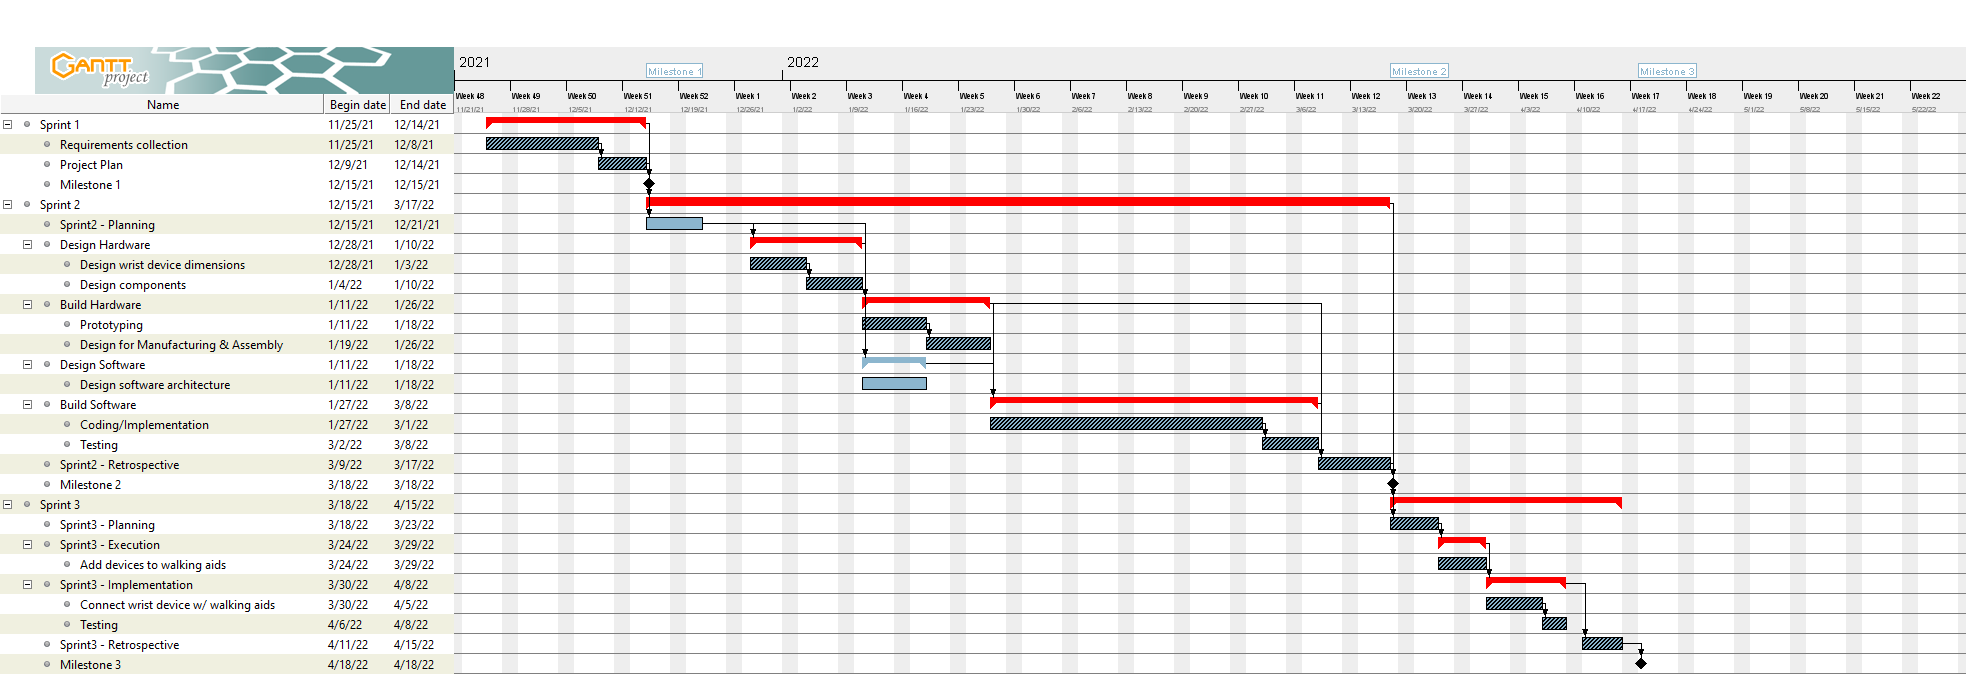
\includegraphics[width=1.0\linewidth]{graphics/ganttm1.png}

% Caption is defined with a short and long version. The short version is shown in the
% List of Figures section, and the long version is used directly with the figure.
	\caption[Milestone 1 Gantt Chart]{Our original Gantt chart schedule from Milestone 1 \cite{coaker}}

% For figures label should be defined after the caption to ensure proper figure numbering.
	\label{fig:ganttm1}

\end{figure}
                
                We attempted to solve these issues by trying to order our hardware after the Christmas period and by attempting to complete our Milestone 1 document within a week of the deadline. Had we made our sprints shorter, we could have created a more proactive mindset within the team to complete these pieces of work sooner and ultimately save time to develop the project further in future. To ensure that we did not face these issues for the remaining time of the project, we decided to make our sprints shorter for the Gantt chart schedule that we included in our Milestone 2 document \cite{mile2}. This Gantt chart demonstrates the conscious effort we made to shorten our sprints and attempt to create a more proactive mindset within the team by encouraging the team to advance the project sufficiently for each sprint deadline. Figure \ref{fig:ganttm2} demonstrates this Gantt chart.

                % [H] means put the figure HERE, directly when you input this code.
\begin{figure}[H]
	\centering
	\captionsetup{width=1.0\linewidth}

% We set the width of the figure based on the width of one line of text on the page.
% The value can be tuned to any value in [0.0, 1.0] to scale the image while maintaining its aspect ratio.

	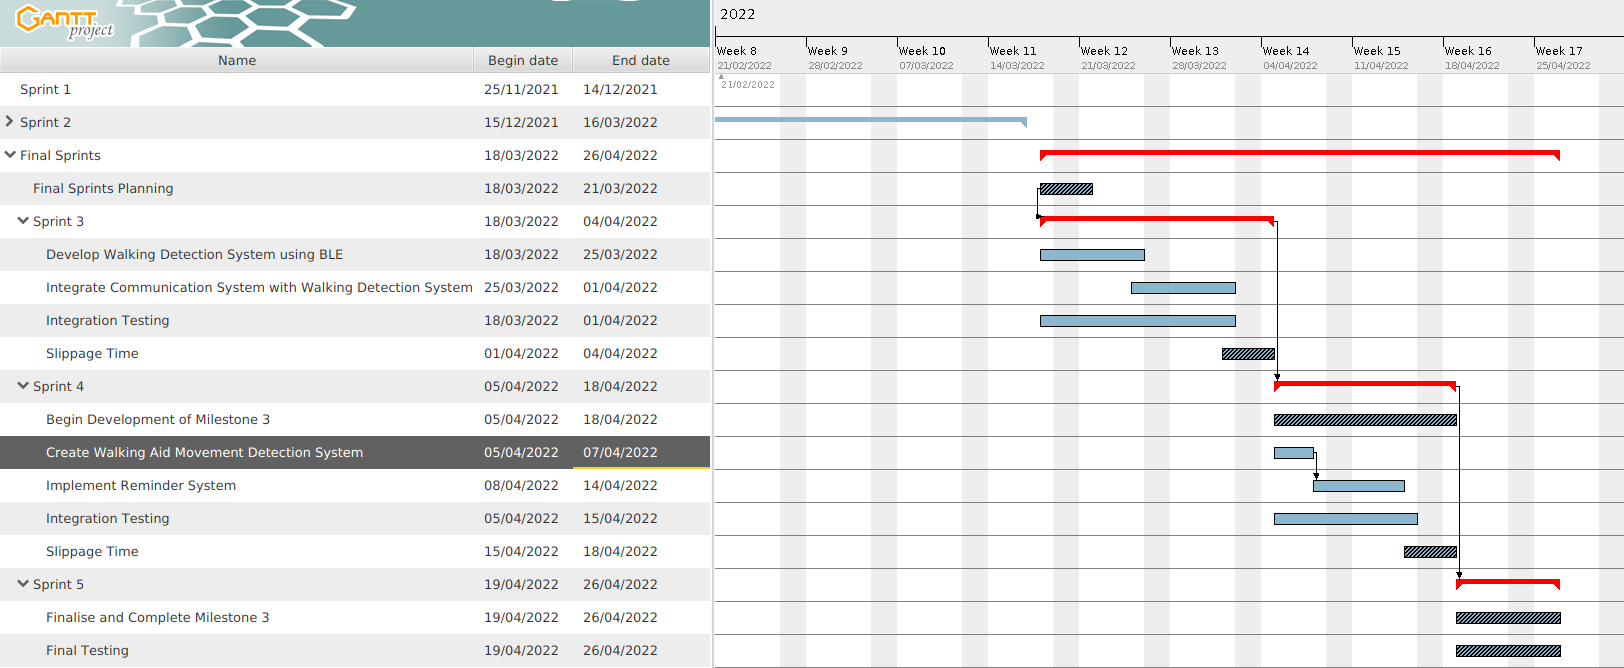
\includegraphics[width=1.0\linewidth]{graphics/ganttm2.png}

% Caption is defined with a short and long version. The short version is shown in the
% List of Figures section, and the long version is used directly with the figure.
	\caption[Milestone 2 Gantt Chart]{Our updated Gantt chart schedule from Milestone 2 \cite{mile2}}

% For figures label should be defined after the caption to ensure proper figure numbering.
	\label{fig:ganttm2}

\end{figure}

                Upon adjusting our second Gantt chart, we noticed that our team was more actively attempting to progress the project with each passing sprint. Having said this, it would be interesting to monitor the activity of the team had both schedules been compared at similar stages of the project's lifecycle. We say this as it is a fair assumption that the project might also have progressed more consistently in the latter stages of its lifecycle since the team were more pressured as the project deadline approached.

            \subsubsection{Hardware Procurement}
            \label{subsec:hardware_procurement}

                As mentioned in our previous Milestone 2 document \cite{mile2}, we experienced delays in the procurement of hardware devices necessary to develop the project. These delays resulted in the delays in beginning code development, which ultimately left us in a position of having limited time to complete the project and not enough time to test all the potential technologies that we could have used. Hardware delivery delays occurred due to the complex process required to be completed to order hardware through the University, as well as courier delays taking place. Having said this, we could have limited the likelihood of this issue occurring by having the team prioritise the hardware procurement process earlier in the lifecycle of the project. Ultimately, we should have foreseen potential delays over the Christmas and New Year period and ensured that we had our hardware orders sorted before the University closed for Christmas. 

                Without the benefits of hindsight, we attempted to complete the work we could complete without the full hardware inventory which allowed us to save time later on in the project lifecycle to develop the other features. As we already had an inventory of 2 TinyPICO boards, we were able to implement the communication protocol whilst waiting for the delivery of the full hardware inventory. This meant that when the full inventory was delivered, we could focus our attention on the development of the other features, such as movement detection and the audio system in the walking aid device. This solution worked well and certainly eased the pressure when developing the other features of our systems. However, had we managed to order our hardware earlier, we could have started to implement the stretch goals supplied to us that would have advanced the project to the next level.

            \subsubsection{Lack of a Team Leader}

                Before beginning the process of developing this project, we were encouraged to avoid selecting a team lead, which was understandable as this is a student project where all group members are expected to contribute an equal amount. However, we found that not having a team leader might have been detrimental to the overall work ethic of the team. One member attempted to take a team leader role implicitly by trying to lead by example with the amount of work they were committing to the git repository. Unfortunately, this seemed to have still led to a negative outcome where some team members were potentially avoiding completing work with the confidence that the leading team member would continue to complete the work instead. Because of this, the progress of the project was certainly negatively affected with some features and documents needing to be rushed. Having said this, the solution that the implicit team leader attempted certainly advanced the progress of the project and ultimately still managed to push the project to a point where the team feel that it is complete and meets the requirements specified in the Milestone 1 document \cite{coaker}.

            \subsubsection{Non-Functional I\textsuperscript{2}C Communication in ADXL345 Library}
            \label{subsubsec:ADXL}

                When developing the initial code for retrieving readings from the ADXL accelerometer, we were instantly limited to using I\textsuperscript{2}C communication rather than SPI communication as the SPI communication technology was being occupied by the audio shield within the walking aid device. However, we noticed that the library we were using was failing to communicate with the accelerometer effectively over I\textsuperscript{2}C. Due to the developer's previous experience in working with I\textsuperscript{2}C, we were able to identify an unnecessary line of the code in the library that was limiting the communication to the accelerometer from working. The original function that we needed to edit can be seen in figure \ref{lst:old_accel}.

                \lstinputlisting[language=C++, caption=The original erroneous function within the accelerometer library., label=lst:old_accel]{listings/old_accel_lib.cpp}

                The line of code that was causing the error was the extra unnecessary beginTransmission call that was included in line 8. The solution was to simply remove this line of code and the I\textsuperscript{2}C communication system between the TinyPICO and the accelerometer was instantly functional. Having already implemented this fix, we later identified that a newer version of this library existed on GitHub which fixes this very issue. However, this version was not available on the Arduino libraries manager, so that is why we opted to edit the library ourselves. There are huge benefits to this though, as it gave us first-hand experience of attempting to understand and edit code that was written by other developers. Our solution to this issue can be seen in figure \ref{lst:new_accel}.

                \lstinputlisting[language=C++, caption=Our fixed function edited within the accelerometer library., label=lst:new_accel]{listings/new_accel_lib.cpp}

            \subsubsection{Inefficient SD Library}
            \label{subsubsec:sd}

                This issue was outlined previously in section \ref{subsec:sdfat}, but we thought we should reiterate it here in a narrative format. When developing the code that allowed the transferral of an audio file from the MicroSD card to the SPIFFS storage space on the TinyPICO development boards we opted to utilise the SD library provided by Arduino. This was because the library was designed as a wrapper for the more complex SdFat library. In essence, we opted to use the Arduino SD library as it looked to be simple to implement and use for our purposes. However, we noticed that the SD library was taking a remarkably long time to read the audio file on the MicroSD card. More specifically, the library was taking 150 seconds to read a 150 KB MP3 file, which was completely unacceptable for our purposes. Upon further investigation, we noticed that many other developers were experiencing a similar issue and were recommending the use of the original SdFat library instead. It took some time to implement this library but once we did, the improvements were astounding. We were able to instantly decrease the read time of the audio file from 150 seconds, down to about 10 seconds. This solution provided a huge improvement in our ability to read the audio file from the MicroSD card and was crucial in the development of our product. This issue did provide a learning opportunity for us, allowing our team to realise that research should be done into libraries before utilising them, and to not always select the library that seems the easiest to implement at the time.

            \subsubsection{Vibrator Limitations}

                The mobile coin cell vibrator made available to us was simply too high powered and would result in damaging our TinyPico's GPIO pins which are limited to 12mA. The vibrators require 70mA to sustain vibration, and even higher to overcome inertia and startup. This wasn't part of the initial scope, however, we already had transistors from previous hobby projects that were suitable to control this, but had to be improvised once the hardware was on hand.


            \subsubsection{Our Chosen Methodology}
            \label{subsubsec:methodology}

                In our Milestone 1 document, we stated that we would follow the Scrum software lifecycle methodology as a means to ensure that we successfully implement the requirements set out in that document \cite{coaker}. However, this software lifecycle methodology did not seem to suit the nature of our project, the work ethic of our team members, or the pressures we faced with deadlines for other University work. The Scrum methodology requires constant input from all team members, who are all working towards completing the same task on a 2 to 4 weekly basis. Our interpretation of the Scrum methodology was to attempt to meet every week, rather than following the daily meeting precedence set by the usual Scrum methodology. We had initially opted for this meeting frequency as it would have been unreasonable to expect full-time students to meet every day to discuss a project. However, with the lack of commitment to meetings from some group members, and with the University curriculum affecting our planning, it was implausible to hold group meetings every week. We also identified that being able to implement features every 2 to 4 weeks as per the Scrum methodology was also implausible, especially when we experienced delays in the procurement of hardware, but also since group members were working on different schedules and were not all committed to implementing features in a timely fashion.

                In our Milestone 1 document, we also assigned a Scrum leader who was not assigned as a team leader, but more of an organiser of the development of the project \cite{coaker}. It was originally planned that the Scrum leader would implement the methodology and ensure that the team were on the same page throughout the development of the project. However, due to the complacency of some group members, the Scrum leader ultimately implemented the majority of the work for this project. In some ways, this could be seen as a solution to the problem outlined here, as this allowed the work of the project to be completed on time and to what we feel is a high standard. Having said this, it did not solve the issue of attaining equal contribution from all group members and a potentially better solution would have been to reinstate a Scrum leader for each Milestone of the project. This would have given group members equal opportunities to lead the Scrum methodology and could have created a work ethic that promoted equal contribution throughout the team.

        \subsection{Concluding Remarks}

            To conclude, we feel that the project was a success overall. We managed to implement the requirements that were agreed upon at the beginning of the project's lifecycle. We certainly feel that issues that we faced along the way limited the overall outcome of the project and effectively restricted our team from being able to implement stretch goals on time, and test the system with different technologies to identify the optimal makeup of the system. Many of those issues were self-inflicted, and we feel that many of the issues could have been avoided had we made an effort as a team to be more proactive. For example, the ordering of devices as soon as possible could have avoided the delays that we experienced, and using time management to develop parts of our documentation whilst waiting for code to be developed could have left more time for code development closer to the project deadline. Having said this, the project is certainly as successful as we hoped it would be, and we feel confident that the product that we have developed can provide the basis of technology that can improve the quality of life of dementia patients and their carers in future. We believe that what we have developed here provides an insight into how such devices can be developed with a short time frame, and minimal budget, and hope that it can be advantageous to the developers that take this project on board when we hand it over to the client.

    
    \section{Reflective Remarks}

        The following section will include a reflective account of the overall project. This will include details on what skills and lessons we learned from the project, what we would have done differently had we been given more time and a larger budget, what we would do differently if the project were to be repeated, before a reflection on how we worked as a group and how well we worked with the client. Finally, we will include an evaluation of our risk analysis section that was previously updated in our Milestone 2 document \cite{mile2}.

        \subsection{Risk Analysis Evaluation}
        \label{subsec:risk}

            This section will include our previously updated risk analysis table from the Milestone 2 document \cite{mile2}. This time around, we will include a body of text along with each risk that arose during the project, which states how specifically went about minimising the risk. Fortunately, we did not experience any risks after the submission of our updated risk analysis section, therefore all risks identified within this section were included in the Milestone 2 document \cite{mile2}. Following the table of risks and solutions we used to minimise the impact of those risks, we will conclude by evaluating how well our previously defined mitigation strategies worked in minimising the impact of the risks.

            \afterpage{%
                \clearpage% Flush earlier floats (otherwise order might not be correct)
                \thispagestyle{empty}% empty page style (?)
                \begin{landscape}% Landscape page
                    \centering % Center table
                    \small
\begin{xltabular}[H]{\textwidth}{c | X | X}
    \caption[Risks Table]{A table of risks along with strategies to mitigate those risks.}\\

    \toprule

    Code & Risk & Mitigation\\

    \midrule
    \endfirsthead

    \toprule

    Code & Risk & Mitigation\\

    \midrule
    \endhead

    \hline
    \multicolumn{3}{|r|}{{Continued on next page}}\\
    \hline
    \endfoot

    \bottomrule
    \endlastfoot

    RSK1

    &

    Our hardware devices may fail and will limit development and testing.

    &

    To mitigate this risk we will choose to use low cost but still effective hardware, which will allow for extra funds within our £150 budget should we need it to replace hardware during development. We also have the opportunity to attain TinyPICO devices from the University for this project, allowing us to minimise the effects on our budget. \textbf{The processes for ordering and funding replacement hardware should be known in advance of the event of any piece of hardware being broken. }\\

    \midrule

    RSK2

    &

    The Rx/Tx modules could fail disabling communication between the wearable and walking aid devices.

    &

    The replacement of these modules should not be much of an issue due to their low cost. The real issue would arise when an Rx/Tx module fails whilst in operation for a patient. We would need to form a protocol here that detects when communication is unable to occur between the 2 devices, and can alert the patient's carer of this.\\

    \midrule

    RSK3

    &

    Uploading erroneous code to our TinyPICO devices could brick the TinyPICO devices.

    &

    Should this occur, we could attempt to reflash previosuly working code onto the TinyPICO. If this fails, we would be left with the occurrence of risk RSK1 where we would need to replace the TinyPICO devices that have been bricked. The low cost of the TinyPICO devices should enable us to purchase some replacements if need be.\\

    \midrule

    RSK4

    &

    GitHub experience a malicious attack or a server failure which could cause our repository to be lost.

    &

    Mitigating this risk is difficult. It's unlikely this will happen and that we would lose our repository as GitHub likely uses a vast backup storage solution. But, should it happen it would be catastrophic and so we should mitigate against this risk. To do this, each developer within the team will store a clone of the repository on their personal system and the team will be able to piece the code back together should this risk arise.\\

    \midrule

    RSK5

    &

    The user requirements we accept could be too large to implement within the given time frame for the project, potentially leaving the client disappointed at project handover.

    &

    To mitigate against this risk, we have discussed our user requirements with the clients and feel that we have decided upon a set of features that we feel we can confidently implement within the time frame given to us. We have also some marked some features as stretch goals to ensure that the most important features are added first. \textbf{There will be frequent communication between group members to ensure everyone is aware of progress and any delays that might affect feature implementation.}\\

    \midrule

    RSK6

    &

    University commitments could impact the development and testing of the product.

    &

    We have attempted to account for this within our schedule by allowing for slippage. Slippage time could allow for the development of unfinished features. We could also spread unfinished work between developers as extra work in an attempt to complete the development of features on time. \textbf{Testing should be planned in advance when group members have time, so that when the testing needs to be carried out, it can be done quickly and efficiently. We are planning to run integration testing now throughout the remaining development of the project.}\\

    \midrule

    RSK7

    &

    The hardware we choose to use may lack the libraries and compatibility with other hardware for quality feature development.

    &

    To avoid this, we will select hardware that is compatible with the Arduino ecosystem to ensure that they are compatible with each other and that libraries are available for code development.\\

    \midrule

    RSK8

    &

    Natural disasters could bring about the loss of hardware and software being used for the development of our product.

    &

    The use of low cost hardware in this system will allow us to replace any compromised hardware if need be. We have decided to store the team's code in a GitHub repository which will allow our code to be protected in an off cite facility. The loss of developer computer systems is by far the biggest risk here, as our budget would not be able to cover the replacement of such computer systems.\\

    \midrule

    RSK9

    &

    Especially in the current coronavirus climate, our developers may be unwell for a period of time that has a negative impact on the development of the project.

    &

    Within our schedule we have included time for slippage that should allow for any time needed by the team to be taken off due to illness. Should a developer need to self isolate and should they not be experiencing symptoms, they could continue to work on the product from a remote location using the GitHub repository.\\

    \midrule

    RSK10

    &

    An Inadequate testing strategy could allow unidentified bugs to be released in the product when handing it over to the client. This could lead to a disappointed client.

    &

    To mitigate against this risk we have devised a testing strategy that ensures thorough testing is carried out throughout the development of our product. We are confident that the proposed testing strategy will allow the team to identify and correct errors in the system before the product is released to the client. \\

    \midrule

    RSK11

    &

    Poorly developed code could mean that despite substantial testing, many bugs could still be included in the product at the conclusion of the project lifecycle, leaving our product to be ineffective for the uses that the client requires.

    &

    To mitigate this risk, we will be following our testing strategy outlined in this document to allow for integration testing. This means that testing will take place every time a new feature is added to the system, allowing us to detect bugs quickly as features are implemented. \textbf{Code should be reviewed by another group member to aid in spotting any major bugs or errors.}\\

    \midrule

    RSK12

    &

    The wearable device we create may cause patients to feel uncomfortable limiting their use of the device.

    &

    We are slightly out of control with this risk as it mainly depends on how the patient reacts to the wearable. Having said this, we aim to make the wearable as discrete and as watch like as possible in an attempt to avoid the patient feeling uncomfortable when wearing it.\\

    \midrule

    RSK13

    &

    Our device could startle or scare the patient putting them in danger.

    &

    We have taken on board the advice of the client for this risk and will be ensuring the watch does not use vibrations or LEDs unless the patient is deaf. We will ensure that generic alarms are not used also in an attempt to avoid startling the patient.\\

    \midrule

    RSK14

    &

    One of our developers could leave the institution, lowering the number of developers we have available to work on the project.

    &

    Should this occur, we would definitely need to use the slippage time we have allowed for in our schedule. We would not be able to bring another developer into the team and would therefore need to share the workload of the developer that is leaving to the other developers on the team. \textbf{We will ensure that all of the group are familiar with what each other is doing, so that in the need to take over from a member on short notice, the transition will be quick, and seamless.}\\
    
    \midrule

    \textbf{RSK15}

    &

    \textbf{Delays in ordering replacement hardware could cause the project to fall irreparably behind schedule.}

    &

   \textbf{Steps to mitigate RSK1 and RSK3 should be followed. To minimise chances of "bricking" hardware, permanent, difficult to undo processes should only be completed when necessary and the system relying on those parts has been properly tested to ensure no damage will occur. We have also already acquired multiple sets of devices to ensure that we have fallback hardware if necessary.} \\
   
    \midrule

    \textbf{RSK16}

    &

    \textbf{Due to previous delays, insufficient time to adequately complete the project.}

    &

   \textbf{Frequent communications and meetings should be held to ensure the group are familiar with the current status of the project, with weekly meetings already being booked, and how well the project is following the agreed upon time plan. In the event of falling behind irreparably, communication with the client is important to ensure that the product produced is as useful as possible.}\\

\end{xltabular}
\label{tbl:risk_table}

                \end{landscape}
                \clearpage% Flush page
            }

            \newpage

            Seeing that we only needed to apply solutions to 5 out of 16 identified risks, we feel that our previous risk analysis was successful and certainly benefited the project. The solutions that we applied when some identified risks did occur were all successful and allowed the project to be completed on time despite project progress being hampered by the occurrences of illness, hardware procurement delays and University work that was large enough to negatively affect the progress of the project. 

            We updated our risk analysis section in Milestone 2 \cite{mile2} to include risks that we had not previously identified in our Milestone 1 document \cite{coaker}, but since the submission of our risk analysis section, we have not seen the occurrence of any unidentified risks. Because of this, we feel that our risk analysis work throughout this project's lifecycle has been successful and led to a situation where unidentified risks did not arise during the most crucial stages of project development.

            Having said this, the fact that we failed to identify risks in the area of hardware delivery delays was certainly detrimental to the progress of this project. We can only put this down to naivety and lack of experience in working on hardware projects, but it meant that not enough attention was paid early on in procuring hardware and meant that significant delays were experienced before the team could even begin developing fundamental features of the project. In future, identifying and analysing risks such as these within hardware projects are crucial in ensuring that the progress was a success. We were fortunate with this project, as team members' experience with similar hardware ensured that our software systems could be developed in time. In future, this may not be the case.

        \subsection{Learned Skills and Lessons}

            This section will detail any skills and lessons that we learned throughout the development of this project.

            \subsubsection{Communicating with a client}

                For some group members, this was the first project where they had the opportunity to work with a client in developing a software project. The biggest lesson that we learnt from this, is how important it is to guide the project in a direction that suits the team members' skill sets. After our introductory meeting with the client, we left with the client stating that they would be content with the project going in one of two directions. It was at this point that we received some advice from our supervisor to take control of the project and guide the client to select the direction that best suited the capabilities and experience of our team members. In our second meeting with the client, we did just that. We explained how we felt that the direction of building movement detection devices with accelerometers would benefit the outcome of the project and would allow us to build a solution to the best of our abilities. The client happily accepted and that was the direction the project followed throughout.
                
                The other lesson we learnt was the importance of keeping frequent contact with the client. This ensured that the client was informed of the progress of the project throughout, and we gave the client many opportunities to adjust the project if they felt that they needed to.

            \subsubsection{Identifying and Editing Libraries}

                As mentioned in sections \ref{subsubsec:ADXL} and \ref{subsubsec:sd}, we did experience some issues with libraries that we utilised throughout the project, with the first SD library we implemented being inefficient, and the I\textsuperscript{2}C code of the ADXL library we used being non-functional. The process of developing this code allowed us to edit other developers' libraries, furthering our experience of code understanding and development, in the instance of fixing the non-functional ADXL. In the case of the inefficient SD library, we learnt the importance of identifying the most appropriate libraries for our needs, rather than instantly opting to use the most simple library to implement. Learning this should allow us to save valuable time in code development for future projects.
                Further information on the code we changed and the issues that we faced with libraries can be viewed in the aforementioned sections.

            \subsubsection{Developing code with Doxygen in mind}

                As we were required to include documentation of our software within this document, we realised that we needed to design our code such that it could be documented effectively using Doxygen, a documentation API tool. This meant that we improved our skills in breaking up our code into multiple classes that each have their purpose in the system. Adopting this way of coding allowed us to develop our understanding and experience of coding with other developers in mind. That is, we assume that other developers will take on this project in future, and we designed the code with them in mind, by trying to make the code as readable and understandable as possible.

                Once we had completed the development of the software, we turned our attention to developing the documentation of our code. Utilising Doxygen was a new learning curve for us, but it provided a solid solution to developing a documentation API of the code we produced, which can be handed on to the future developers of this project with ease. As well as this, we followed the LaTeX documentation format that Doxygen creates to include documentation of our software within this document. The experiences we have had here will stand us in good stead when developing software in the industry. Evidence of our documentation and class structures can be seen in sections \ref{sec:class_documentation_walk_aid} and \ref{sec:class_documentation_wearable}.

            \subsubsection{Developing UML Diagrams with Umbrello}

                The team have had previous experience in creating class diagrams as a basis for demonstrating the design of our software systems in previous University work. However, the development of UML diagrams in Umbrello was new to us, as well as the development of activity diagrams in general. We had previously aimed to include flowcharts within this document that demonstrated the workflow of our software systems but realised that activity diagrams do this well and are a part of the UML diagram family. Therefore, we opted to provide activity diagrams within this document instead to illustrate the workflows of our software systems.

                The experiences we have had with utilising Umbrello to develop UML diagrams, and the experiences of developing UML diagrams, in general, will certainly benefit our team members when they use similar methods of documentation in future work. Evidence of our UML diagrams can be seen in chapter \ref{ch:design}.

            \subsubsection{3D Design with internal components and wiring}

                Although members of the team had previous experience with 3D design, they were not familiar with designing with multiple PCBs and components in mind, as well as accounting for the order of operations for assembly. Whilst going through design iterations, it became clearer how the housings had to be designed, to allow them to be easily assembled and disassembled. One time where this lack of knowledge became apparent was during the assembly of the mid-housing for the walking aid device, where the speaker wires had to be initially connected to the AudioShield, as the TinyPico would obscure it when in place. This caused some issues during initial assembly, but has since been rectified in later designs. Regardless, designing with tolerances for wiring and soldering is something new to the team, and a valuable skill to carry into the industry and other personal hobbies.
                
        \subsection{What if there was more time and a larger budget?}

            As previously mentioned in this document, we feel that we were able to fulfil all client requirements with this project, however, we had to omit some stretch goals to allow for the main requirements to be met. Therefore, had we been assigned more time to complete this project, or had we managed to sort hardware procurement sooner, we certainly would have attempted to implement a fall detection feature into our wearable device, as well as a battery powering feature for both devices. As well as this, we would have liked to have tested Bluetooth distance measurement between the devices as a means for movement detection to identify if it had been more useful than our current solution which monitors changes in gravity. We had stated in our Milestone 2 document \cite{mile2} that we would test this within the timeframe of this project, but unfortunately, we were unable to complete the software for this test feature in time. The features that we would have liked to have included in this project can certainly be completed in the future work of this project, and we recommend that the developers that continue this project in the future look into developing these features in an attempt to improve our solution.

            Had we been assigned a larger budget for the project, we would have implemented an ultra-wideband solution for movement detection in the wearable device by measuring distances between the walking aid and wearable device. This would have been implemented and tested against our current solution in a similar way to how we would have liked to implement and test Bluetooth distance monitoring for walking detection. As well as this, we would have liked to have purchased a switch for the walking aid device to allow the patient's carer or relative to switch between audio and vibration reminders depending on the circumstances of the patient. We currently toggle this within the software itself, which is not feasibly for use in a real-world setting, but unfortunately, we could not include switches for the walking aid device within our budget.

        \subsection{What if we could repeat the project?}

            There are particular aspects of this project that we would certainly change if we had the chance to repeat it. The most critical of those is the hardware procurement process that we experienced. As mentioned in section \ref{subsec:risk}, it may have been naivety or our inexperience in hardware projects that led to us not being proactive in the process of ordering necessary hardware for the project. This led to a large amount of time lost that could have been spent developing the project further. If we could repeat the project, we would have ensured that our list of hardware was finalised and ordered as soon as the client agreed to our list of requirements, which in turn could have allowed for a few more weeks worth of development time.

            Alongside this, we would have opted to utilise a different software lifecycle methodology to the Scrum methodology that we chose, such as the Prototyping methodology. Despite the Scrum methodology being an agile methodology, it still assumes that features are implemented every 2 to 4 weeks, and with our original methodology plan stating that we would meet every week, it became too rigid for the type of project we were trying to develop. A better choice might have been to utilise the prototyping methodology and set deadlines with slippages for each prototype to be developed. That way we could have adopted a more agile approach and set deadlines based on how busy team members were with other University work. We could also have planned meetings depending on the progress being made on the prototype, with prototyping also potentially helping to bring about more software contributions from some team members.

            Finally, if we were to repeat the project, we would like to experiment with either assigning a team leader for the whole project or splitting the project into 4 parts and assigning a team leader for each section of the project. We would have liked to experiment with this to see if it would incur a greater and more equal effort and contribution from each group member, which ultimately would have increased the quality of this project and its documentation. As mentioned previously, one group member attempted to lead the group by example with the amount of work they were contributing to the project. However, this did not have the desired effect and potentially helped to create a situation where group members did not contribute equally to this project due to their work having to be done by others for the sake of project completion.

        \subsection{Time Plan Reflection}

            We previously mentioned some issues we faced with our original time plan and schedule in section \ref{subsec:schedule}. In this section, we will reflect on our overall time plan and whether it was useful to us in fulfilling the requirements of this project. 

            \subsubsection{Time Plan from Milestone 1 to Milestone 2}

                Within our Milestone 1 document \cite{coaker}, we submitted a Gantt chart of our schedule for the development of the project from the Milestone 1 deadline up until the overall deadline for the project. We had agreed to follow a Scrum methodology, but unfortunately designed our schedule such that the planned sprints were far too long. Figure \ref{fig:ganttm1-2} illustrates the Gantt chart of our schedule, with the problematic sprints. As we can see, Sprint 2 specifically contains plans for all the work to be carried out to develop the prototypes. This created a situation where the team was unable to identify easily what work needed to be carried out when and left us in a situation where some tasks were not assigned a high enough priority to be completed. For example, had we included shorter sprints in our original schedule, we may have assigned a higher priority to the specification and procurement of hardware necessary to implement the project. Having shorter sprints could also have allowed us to hold team members more accountable for lack of contribution, as we would have been able to scrutinise when specific features should have been implemented and why they were not implemented on time. Having said this, as previously stated, we did experience issues with utilising the Scrum methodology within this project's lifecycle and so minimising the duration of each sprint may not have improved the overall progress made between the submission of the Milestone 1 and Milestone 2 documents (December 14th and March 18th).

                It can also be noticed that a distinct lack of explicit slippage time was included within our Gantt chart in Milestone 1 \cite{coaker}. Slippage time was crucial in allowing us to implement our features on time between the submission of our Milestone 2 document and the deadline for the project. Therefore, omitting explicit slippage time from our original schedule could have been detrimental to the progress of the project, and may have put our team members under distinct pressure to complete features on a strict time plan.

                % [H] means put the figure HERE, directly when you input this code.
\begin{figure}[H]
	\centering
	\captionsetup{width=1.0\linewidth}

% We set the width of the figure based on the width of one line of text on the page.
% The value can be tuned to any value in [0.0, 1.0] to scale the image while maintaining its aspect ratio.

	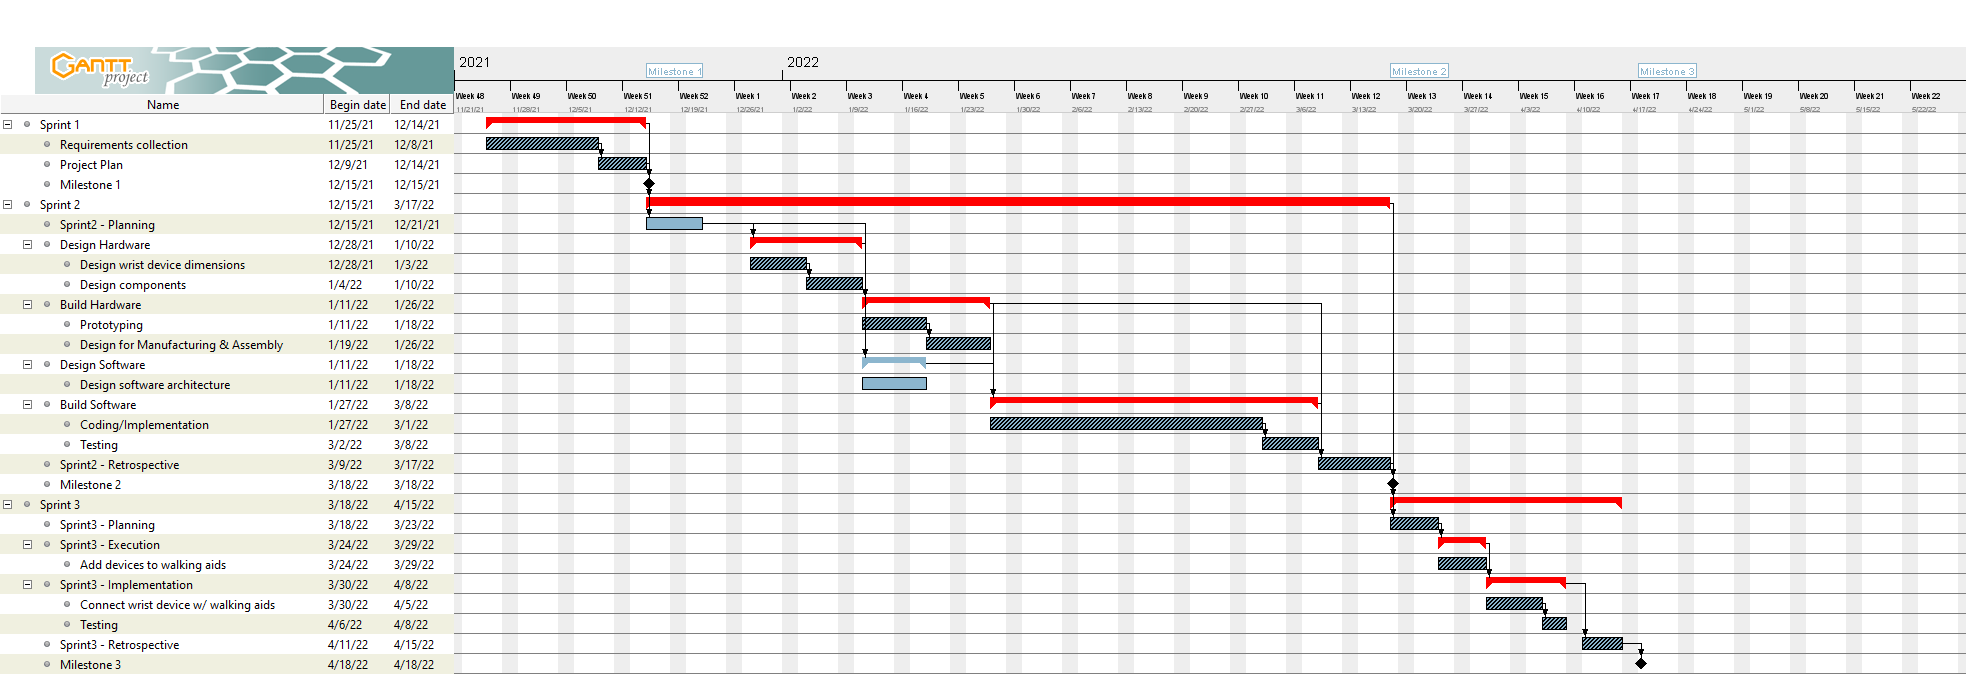
\includegraphics[width=1.0\linewidth]{graphics/ganttm1.png}

% Caption is defined with a short and long version. The short version is shown in the
% List of Figures section, and the long version is used directly with the figure.
	\caption[Milestone 1 Gantt Chart]{Our original Gantt chart schedule from Milestone 1 \cite{coaker}}

% For figures label should be defined after the caption to ensure proper figure numbering.
	\label{fig:ganttm1-2}

\end{figure}

            \subsubsection{Time Plan from Milestone 2 to Project Completion}
        
                Our updated Gantt chart schedule submitted along with our Milestone 2 document \cite{mile2}, was far more successful in allowing the team to monitor the progress of the project and in easing the understanding of what features still needed to be completed by the project deadline. Figure \ref{fig:ganttm2-2} illustrates how we adjusted our schedule to include shorter sprints, a week or two for each, in the hopes that it would fuel higher contribution from the team towards the development of the project. While we feel that shorter sprints may have contributed to the more rapid progress of the project's development, when being compared to the progress made with our original schedule, the improvement of progress rates between the submission of the Milestone 2 document and the project deadline might also have been caused by the pressure applied to the team by an approaching final deadline.

                The slippage time explicitly included in our updated Gantt chart in Figure \ref{fig:ganttm2-2} was crucial in ensuring that the development of features was commenced early, but that some features could continue to be developed during the slippage time if need be. This increased the quality of the features and documents developed between March 18th and April 26th. The allowance for the testing time after each sprint allowed the team to ensure that the devices were functional and that the development of the next sprint could begin confidently. 

                % [H] means put the figure HERE, directly when you input this code.
\begin{figure}[H]
	\centering
	\captionsetup{width=1.0\linewidth}

% We set the width of the figure based on the width of one line of text on the page.
% The value can be tuned to any value in [0.0, 1.0] to scale the image while maintaining its aspect ratio.

	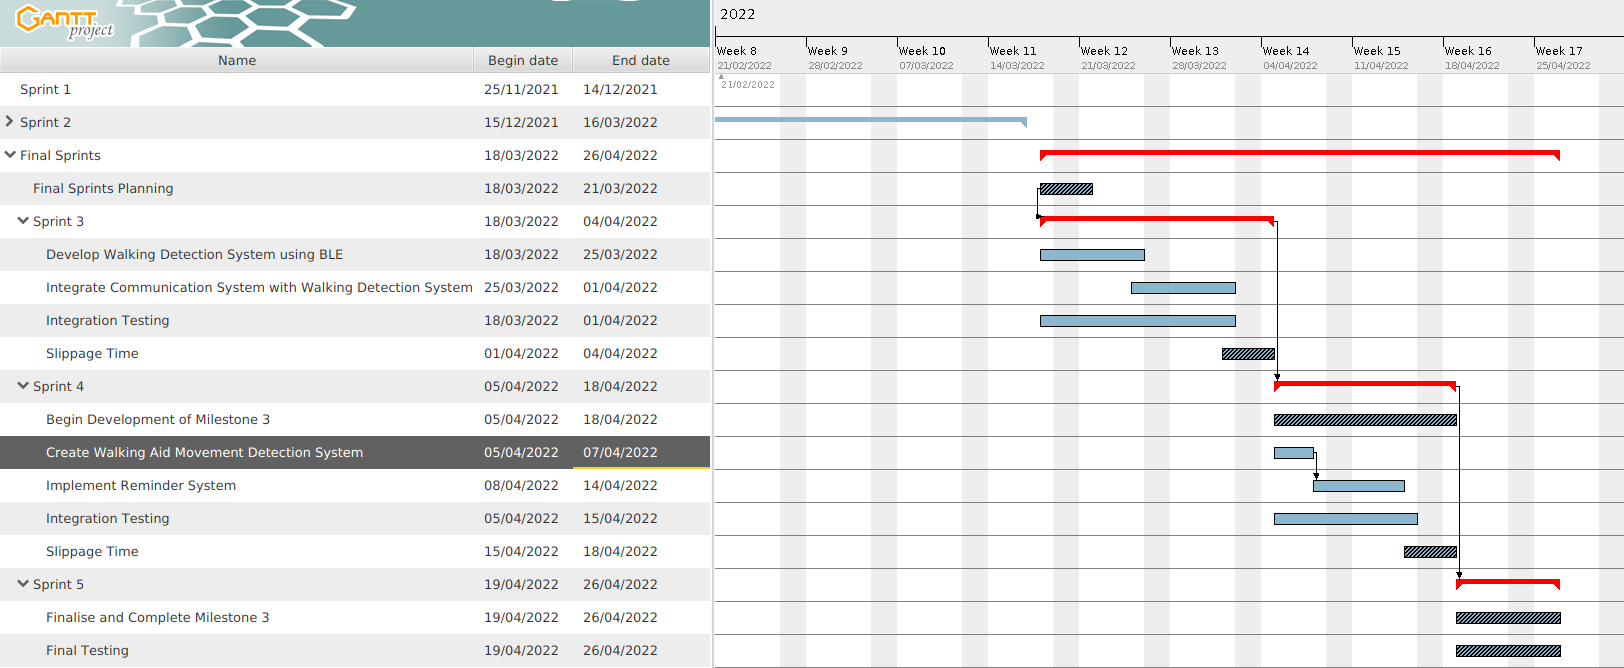
\includegraphics[width=1.0\linewidth]{graphics/ganttm2.png}

% Caption is defined with a short and long version. The short version is shown in the
% List of Figures section, and the long version is used directly with the figure.
	\caption[Milestone 2 Gantt Chart]{Our updated Gantt chart schedule from Milestone 2 \cite{mile2}}

% For figures label should be defined after the caption to ensure proper figure numbering.
	\label{fig:ganttm2-2}

\end{figure}

        \subsection{Team Work}

            Unfortunately, the teamwork throughout the development of this product was not completely fair and equal, with some members contributing more to software and hardware development, and more to the documentation. This section will outline the work each member did towards the development of this project, providing evidence as to how the contribution levels of each team member were not equal. The following will contain a paragraph for each team member, outlining the work they carried out for this project before we finally include an illustration of contribution to our git repository. Our git repository was our main storage location for our documentation and coding work throughout the project. It should be noted, that not all work has been uploaded to our git repository, such as our CAD designs and 3D printing work.

            \subsubsection{Team Member Contributions}

                \paragraph{Sean Coaker}\mbox{}

                Sean took on the role of the communications officer and scrum master, and was therefore responsible for the contact between the team and the client, as well as being responsible for ensuring that work was being completed on time. He contributed heavily to all Milestones that were submitted for this project, with large amounts of content being written for the design (which included all UML and documentation sections), user manual, testing, and narrative and reflective account sections of this document. Further content was also included in the Milestone 1 and 2 documents, where Sean contributed considerable amounts towards the initial risk analysis and requirements sections, as well as the background research and design discussions that were included in both documents.

                As well as this, Sean developed all the software for both the walking aid and wearable devices and created the documentation and test cases for said software. He also executed the test cases to ensure that our project's software systems were fully operational. On top of this, Sean also soldered his hardware to allow him to progress the project in a timely fashion. Finally, Sean also remained in constant contact with team members to ensure that the team were all well-informed on the progress of the project and how he had designed the software of the systems such that the 3D prints could house the exact wiring he had used to develop the prototypes.

                \paragraph{Pedro Caetano}\mbox{}

                Pedro took on the role of developing the housing for our prototypes due to his experience in this area and contributed to each of the Milestone documents submitted for this project. He utilised his knowledge of hardware to help Sean in compiling a list of hardware to be sent to the client for ordering, before using that same hardware to develop the housing of our prototypes. With the use of CAD designs, 3D rendering and 3D printing, Pedro was able to develop useable housing for our prototypes that demonstrates how our devices could be used and worn in the real world. To complete the housing design work, Pedro also needed to solder the hardware devices that were assigned to him, in a way that would be compatible with the tight spaces and tolerances of the physical enclosures, as well as Panayiotis' test components.

                Aside from this, Pedro contributed to all Milestone documents of the project by mainly carrying out organisation and refactoring work within the Milestone 1 document, by including details on the housing of the walking aid device in the Milestone 2 document, before finally including the full design details of the housing of both devices in this document. Pedro alongside Sean, prepared the documentation for submission, ensuring the writing style, format and layout were suitable for the target audience and covered the areas required by the CSCM04 specification.

                \paragraph{Panayiotis Melios}\mbox{}

                Panayiotis contributed to all Milestone documents submitted as part of this project. For the Milestone 1 document, Panayiotis developed our initial schedule within a Gantt chart to demonstrate our time plan for the project. As well as this, he developed a specification section based on the requirements detailed by Sean and agreed to by the client. The Milestone 2 document saw Panayiotis provide work towards updating our schedule from the Milestone 1 document as well as working towards providing a progress report on how much each of the previously detailed requirements had been completed. Panayiotis contributed to this document by helping provide the content to be included within this narrative and reflective account section, as well as creating the poster to be displayed during the demonstration of our project. Panayiotis also attended all intra-group and client meetings throughout this process. 

                \paragraph{Matthew Culley}\mbox{}

                For this project, Matthew contributed by adding content to the Milestone 1 and 2 documents. Matthew provided the content within the methodology section of the Milestone 1 document, as well as providing some background research into the dangers of falling to dementia patients, and ultimately why this project was so important. The risk analysis update section was provided by Matthew for Milestone 2, where he detailed any changes in risks, any risks that had arisen that we had omitted from Milestone 2, and amendments to our mitigation strategies and likelihood/impact risk matrix.

            \subsubsection{Git Repository Contribution Summary}

                The following illustration in figure \ref{fig:git}, demonstrates the contribution of each group member to the project's git repository, the main storage location for software and documentation required to complete this project. It should be noted that not all work has been uploaded to the git repository such as 3D modelling and rendering work and that some contributions may seem larger as those team members submitted Doxygen generated documentation to the git repository.

                % [H] means put the figure HERE, directly when you input this code.
\begin{figure}[H]
	\centering
	\captionsetup{width=1.0\linewidth}

% We set the width of the figure based on the width of one line of text on the page.
% The value can be tuned to any value in [0.0, 1.0] to scale the image while maintaining its aspect ratio.

	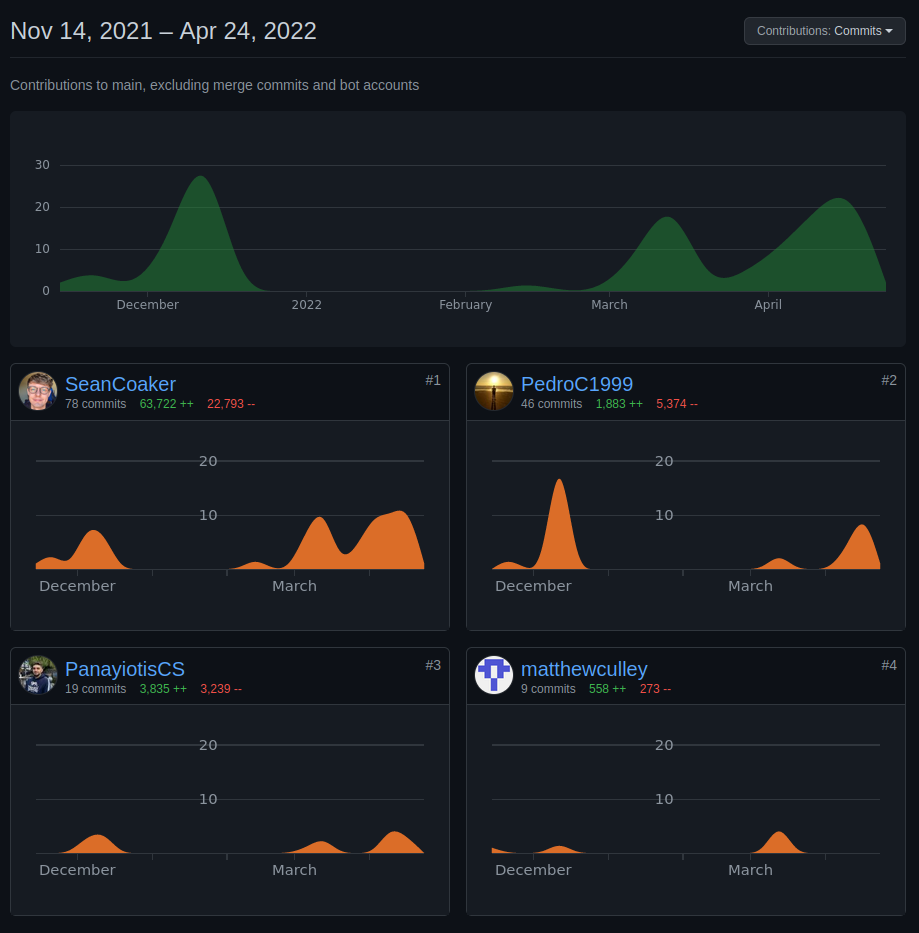
\includegraphics[width=1.0\linewidth]{graphics/git_contributions.png}

% Caption is defined with a short and long version. The short version is shown in the
% List of Figures section, and the long version is used directly with the figure.
	\caption[Git Repository Contributions]{An illustration of how each group member contributed to the project.}

% For figures label should be defined after the caption to ensure proper figure numbering.
	\label{fig:git}

\end{figure}